\newcommand{\lecturetitle}[1]{
  \title{01204211 Discrete Mathematics \\ #1}
  \author{Jittat Fakcharoenphol}
  \frame{\titlepage}
}

\lecturetitle{Lecture 15: Fibonacci sequence} 

\begin{frame}\frametitle{The Fibonacci sequence\footnote{This lecture mostly follows Chapter 4 of [LPV].}}

  \begin{columns}[c]
    \column{.3\textwidth}
    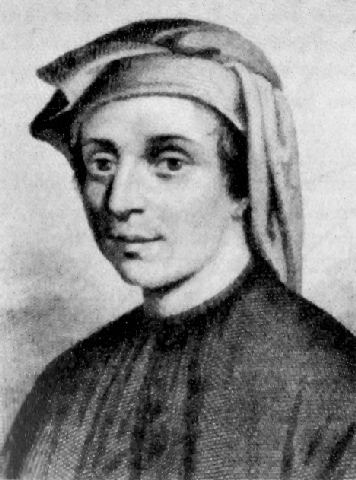
\includegraphics{images/fibonacci.jpg}

    {\tiny Source: https://en.wikipedia.org/wiki/ File:Fibonacci.jpg}
    
    \column{.7\textwidth}
    In 1202, Leonardo Bonacci (known as Fibonacci) asked the following
    question.

    \begin{tcolorbox}
      {\footnotesize ``[A]ssuming that: a newly born pair of rabbits,
        one male, one female, are put in a field; rabbits are able to
        mate at the age of one month so that at the end of its second
        month a female can produce another pair of rabbits; rabbits
        never die and a mating pair always produces one new pair (one
        male, one female) every month from the second month on.''

        ``The puzzle that Fibonacci posed was: how many pairs will
        there be in one year?''}
    \end{tcolorbox}
    
    {\tiny From https://en.wikipedia.org/wiki/Fibonacci\_number}
  \end{columns}
\end{frame}

\begin{frame}
  Let's try to solve Fibonacci's question. \pause

  Let $\spadesuit$ denote a newly born rabit pair, and $\heartsuit$
  denote a mature rabit pair.
  
  \begin{tabular}{c|l|r}
    Month & Rabits & \\ \hline
    1 & $\spadesuit$ & 1 \\ \pause
    2 & $\heartsuit$ & 1\\ \pause
    3 & $\heartsuit$ \pause $\spadesuit$ & 2 \\ \pause
    4 & $\heartsuit$ $\heartsuit$ \pause $\spadesuit$ & 3 \\ \pause
    5 & $\heartsuit$ $\heartsuit$ $\heartsuit$ \pause $\spadesuit$ $\spadesuit$ & 5 \\ \pause
    6 & $\heartsuit$ $\heartsuit$ $\heartsuit$ $\heartsuit$ $\heartsuit$ \pause $\spadesuit$ $\spadesuit$ $\spadesuit$ & 8 \\ \pause
    7 & $\heartsuit$ $\heartsuit$ $\heartsuit$ $\heartsuit$ $\heartsuit$ $\heartsuit$ $\heartsuit$ $\heartsuit$
    \pause $\spadesuit$ $\spadesuit$ $\spadesuit$  $\spadesuit$ $\spadesuit$ & 13
  \end{tabular}

  \vspace{0.1in}
  
  \pause How many rabit pairs do we have at the beginning of the 8th
  month? \pause

  {\small
    \begin{itemize}
    \item
      Surely all 13 rabit pairs we have in the 7th month remain there and
      are all mature.  So, the question is how many newly born rabbit
      pairs that we have. \pause
    \item
      The number of newly born rabbit pairs equals the number of mature
      rabbit pairs we have.  \pause This is also equal to the number of
      rabit pairs that we have in the 6th month: 8.
    \end{itemize}
  }
\end{frame}

\begin{frame}
  Thus, we will have 13+8 rabit pairs at the beginning of the 8th
  month.
  \pause
  
  If we write down the sequence, we get the Fibonacci sequence:
  \[
  1,1,2,3,5,8,13,21,\ldots
  \]
  \pause
  Again, what's the next number in this sequence?  How can you compute it? \pause

  21+13 = 34 is the answer. \pause You take the last two numbers and
  add them up to get the next number.  Why? 
\end{frame}

\begin{frame}
  To be precise, let $F_n$ be the $n$-th number in the Fibonacci
  sequence. (That is, $F_1=1, F_2=1, F_3=2, F_4=3$ and so on.)  We can
  define the $(n+1)$-th number as
  \[
  F_{n+1}=F_n+F_{n-1},
  \]
  for $n=2,3,\ldots$.
  \pause
  Is this enough to completely specify the sequence? \pause

  No, because we do not know how to start.  To get the Fibonacci
  sequence, we need to specify two starting values: $F_1=1$ and
  $F_2=1$ as well.

  Now, you can see that the equation and these special values uniquely
  determine the sequence.  It is also convenient to define $F_0=0$ so
  that the equation works for $n=1$.
\end{frame}

\begin{frame}\frametitle{A recurrence}
  The equation
  \[ F_{n+1}=F_n+F_{n-1} \]
  and the initial values $F_0=0$ and $F_1=1$ specify all values of the
  Fibonacci sequence.  With these two initial values, you can use the
  equation to find the value of any number in the sequence.

  This definition is called a {\bf recurrence}.  Instead of defining
  the value of each number in the sequence explicitly, we do so by
  using the values of other numbers in the sequence.
\end{frame}

\begin{frame}\frametitle{Tilings with 1x1 and 2x1 tiles}
  You have a walk way of length $n$ units.  The width of the walk way
  is 1 unit.  You have unlimited supplies of 1x1 tiles and 2x1 tiles.
  Every tile of the same size is indistinguishable.  In how many ways
  can you tile the walk way?

  Let's consider small cases.
  \begin{itemize}
  \item When $n=1$, there are 1 way.
  \item When $n=2$, there are 2 ways.
  \item When $n=3$, there are 3 ways.
  \item When $n=4$, there are 5 ways.
  \end{itemize}

  Let's define $J_n$ to be the number of ways you can tile a walk way
  of length $n$.  From the example above, we know that $J_1=1$ and $J_2=2$.

  Can you find a formula for general $J_n$?
\end{frame}

\begin{frame}\frametitle{Figuring out the recurrence for $J_n$}
  To figure out the general formula for $J_n$, we can think about the
  first choice we can make when tiling a walk way of length $n$.
  There are two choices:
  \begin{itemize}
  \item (1) We can start placing a 1x1 tile at the beginning, or
  \item (2) We can start placing a 2x1 tile at the beginning.
  \end{itemize}

  In each of the cases, let's think about how many ways we can tile
  the rest of the walk way, provided that the first step is made.

  \vspace{0.1in}
  Note that if we start by placing a 1x1 tile, we are left with a walk
  way of length $n-1$.  From the definition of $J_n$, we know that
  there are $J_{n-1}$ ways to tile the rest of the walk way of length
  $n-1$.  Using similar reasoning, we know that if we start with a 2x1
  tile, there are $J_{n-2}$ ways to tile the rest of the walk way.
\end{frame}

\begin{frame}\frametitle{The recurrence for $J_n$}
  \begin{tcolorbox}
    From the discussion, we have that
    \[ J_n = J_{n-1} + J_{n-2}, \]
    where $J_1=1$ and $J_2=2$.
  \end{tcolorbox}

  Note that this is exactly the same recurrence as the Fibonacci
  sequence, but with different initial values.  In fact, we have that
  \[ J_n = F_{n+1}. \]
\end{frame}

\begin{frame}\frametitle{Identities on Fibonacci numbers}
  There are a lot of identities related to Fibonacci numbers.  Let's
  see the first few values in the sequence:
  \[
  0,1,1,2,3,5,8,13,21,34,55,89,\ldots
  \]

  Now, let's add the first few numbers:
  \begin{eqnarray*}
    0+1 &=& 1\\
    0+1+1 &=& 2\\
    0+1+1+2 &=& 4\\
    0+1+1+2+3 &=& 7\\
    0+1+1+2+3+5 &=& 12\\
    0+1+1+2+3+5+8 &=& 20\\
    0+1+1+2+3+5+8+13 &=& 33
  \end{eqnarray*}
  From this we can formulate the following conjecture:
  \[ F_0+F_1+\cdots+F_n = F_{n+2} - 1.\]
\end{frame}

\begin{frame}
  \textcolor{blue}{Theorem:} For $n\geq 0$, we have that \[ F_0+F_1+\cdots+F_n = F_{n+2}-1.\]

  \textcolor{blue}{Proof:} We shall prove by induction on $n$.  The
  base case has already been demonstrated when we consider small
  values of $n$.
  
  \vspace{0.1in}
  {\bf Inductive Step:} Let's assume that the statement is true for $n=k$, for $k\geq 0$, i.e., assume that
  \[ F_0+F_1+\cdots+F_k = F_{k+2}-1.\]
  We shall prove that the statement is true when $n=k+1$.  This is not
  hard to show.  We write
  \begin{eqnarray*}
    (F_0+F_1+\cdots+F_k)+F_{k+1} &=& (F_{k+2}-1) + F_{k+1} \\
    &=& F_{k+3} - 1,
  \end{eqnarray*}
  as required.  Note that the first step follows from the induction
  hypothesis. $\blacksquare$
\end{frame}

\begin{frame}\frametitle{Another harder identity}
  The following identity is harder to prove:
  \[ F_n^2 + F_{n-1}^2 = F_{2n-1}. \]
  Let's try a few values as a sanity check.
  \[
  F_1^2+F_2^2 = 1^2+1^2=2=F_3
  \]
  \[
  F_2^2+F_3^2 = 1^2 + 2^2 = 5 = F_5
  \]
  \[
  F_3^2+F_4^2 = 2^2 + 3^2 = 13 = F_7
  \]

  To see how hard it is to prove the identity, let's try to prove it
  by induction.  (Let's jump to the inductive step.)
\end{frame}

\begin{frame}
  We use strong induction. Assume that the statement is true for
  $n=k,k-1,k-2,\ldots,0$. We prove the statement for $n=k+1$.

  \vspace{0.1in}
  Let's work on the left hand side.
  \begin{eqnarray*}
    F_{k+1}^2 + F_{k}^2 &=&
    \left(F_k+F_{k-1}\right)^2 + \left(F_{k-1}+F_{k-2}\right)^2\\
    &=& F_k^2 + 2F_kF_{k-1} +F_{k-1}^2 + F_{k-1}^2 +  2F_{k-1}F_{k-2} + F_{k-2}^2\\
    &=& (F_k^2 + F_{k-1}^2) + 2F_kF_{k-1} + (F_{k-1}^2 + F_{k-2}^2) + 2F_{k-1}F_{k-2}\\
    &=& F_{2k-1} + F_{2k-3} + 2F_kF_{k-1} + 2F_{k-1}F_{k-2},
  \end{eqnarray*}
  where the last step follows from the induction hypothesis.

  \vspace{0.1in}
  Note that we end up with the terms like:
  $F_kF_{k-1}+F_{k-1}F_{k-2}$.  We can keep expanding the terms, but
  we will end up with the same cross terms like this.

  \vspace{0.1in} So, let's take a look at a few values of this
  expression.  Maybe we can guess its values.
\end{frame}

\begin{frame}
  Let's plug in a few values:
  
  \[ F_3F_2+F_2F_1 = 2\cdot 1 + 1\cdot 1 = 3 = F_4 \] 
  \[ F_4F_3+F_3F_2 = 3\cdot 2 + 2\cdot 1 = 8 = F_6 \] 
  \[ F_5F_4+F_4F_3 = 5\cdot 3 + 3\cdot 2 = 21 = F_8 \] 
  \[ F_6F_5+F_5F_4 = 8\cdot 5 + 5\cdot 3 = 55 = F_{10} \]

  From this, we can make another conjecture:
  \begin{tcolorbox}
    {\bf Conjecture 2:}
    \[
    F_{n+1}F_n + F_nF_{n-1} = F_{2n}.
    \]
  \end{tcolorbox}
\end{frame}

\begin{frame}
  Let's assume that Conjecture 2 is true and see if we can prove the
  identity that we want.

  Recall that we have
  \begin{eqnarray*}
    F_{k+1}^2 + F_{k}^2
    &=& F_{2k-1} + F_{2k-3} + 2F_kF_{k-1} + 2F_{k-1}F_{k-2} \\
    &=& F_{2k-1} + F_{2k-3} + 2(F_kF_{k-1} + F_{k-1}F_{k-2}) \\
    &=& F_{2k-1} + F_{2k-3} + 2F_{2k-2} \ \ \ \ \ \ \mbox{(from Conj 2)}\\
    &=& (F_{2k-1} + F_{2k-2}) + (F_{2k-2} + F_{2k-3})\\
    &=& F_{2k} + F_{2k-1}\\
    &=& F_{2k+1},
  \end{eqnarray*}
  as required.  We use Conjecture 2 to show the second step.

  \vspace{0.1in} This means that assuming the Conjecture 2, we can
  show the identity $F_n^2+F_{n-1}^2 = F_{2n-1}$.
\end{frame}

\begin{frame}\frametitle{Let's prove Conjecture 2}
  {\bf Conjecture 2:} $F_{n+1}F_n + F_nF_{n-1}=F_{2n}$.
  
  {\bf Proof:} Let's do so by induction.  Since we have plugged in
  many small values, we can only consider the inductive step now.
  Assume that the statement is true for $n=k,k-1,k-2,\ldots,0$.  We
  prove the statement for $n=k+1$.

  We write
  \begin{eqnarray*}
    F_{k+2}F_{k+1}+F_{k+1}F_k
    &=& (F_{k+1} + F_k)F_{k+1} + (F_k+F_{k-1})F_k \\
    &=& F_{k+1}^2 + F_kF_{k+1} + F_k^2 + F_{k-1}F_k \\
    &=& (F_kF_{k+1} + F_{k-1}F_k) + F_{k+1}^2 + F_k^2 \\
    &=& F_{2k} + F_{k+1}^2 + F_k^2.
  \end{eqnarray*}
  (Note that the 4th step uses the induction hypothesis.)  Do you see
  any familiar terms?

  \vspace{0.1in} Yes, the terms $F_{k+1}^2 + F_k^2$ is the left hand
  side of the identity we have just proven.  Actually, we cannot use
  it directly here, because we use Conjecture 2 to prove it and now we
  are trying to prove the conjecture itself.  {\bf Using it results in
    a circular reasoning.}
\end{frame}

\begin{frame}
  We can actually prove the conjecture using that identity, but we
  first have to break our circular reasoning by proving both
  statements together.  Formally, let's define predicates $P$ and $Q$:

  \begin{tcolorbox}
    \[P(n): F_n^2 +F_{n-1}^2 = F_{2n-1}\]
    \[Q(n): F_{n+1}F_n + F_nF_{n-1} = F_{2n}\]
  \end{tcolorbox}

  We will prove that for all integer $n\geq 0$, $P(n)\wedge Q(n)$.
    
  {\bf Base Case:} We have shown that $P(1)$ and $Q(1)$ are true.
  
  {\bf Inductive Step:} Assume that the statements are true for
  $n=k,k-1,\ldots,1$ for $k\geq 1$.  We will prove $P(k+1)\wedge
  Q(k+1)$.
  \begin{itemize}
  \item $P(k+1)$ can be proved as in the proof of the identity
    previously.
  \item To prove $Q(k+1)$, we can use the induction hypotheses and
    also $P(k+1)$.
  \end{itemize}
\end{frame}

\begin{frame}\frametitle{Simultaneous induction}
  Let's prove $Q(k+1)$. We can continue from our ``broken'' proof.  We
  have that
  \begin{eqnarray*}
    F_{k+2}F_{k+1}+F_{k+1}F_k
    &=& F_{2k} + (F_{k+1}^2 + F_k^2) \\
    &=& F_{2k} + F_{2k+1} = F_{2k+2},
  \end{eqnarray*}
  as required. Note that the second step uses $P(k+1)$. $\blacksquare$

  \vspace{0.2in}
  The technique we use to prove $P$ and $Q$ together is called {\bf
    simultaneous induction}.
\end{frame}

\begin{frame}\frametitle{An explicit form of the Fibonacci sequence}
  While the recurrence for $F_n$ completely specifies the sequence, it
  is hard to find the value of, say, $F_{20}$ quickly.  We really have
  to enumerate the sequence from $F_0,F_1,\ldots,$ to get to $F_{20}$.
  Also, with the definition based on the recurrence, other properties
  of the sequcen is unclear (e.g., how fast the sequence grows).

  Therefore, it might be useful to find the explicit definition of the
  Fibonacci sequence.
\end{frame}

\begin{frame}\frametitle{Ratios}
  To get started, we might want to look for a common form of the
  function.  We can start by looking at the numbers in the sequence.

  \vspace{0.1in}

  \begin{columns}
    \begin{column}{0.4\textwidth}
      \begin{tabular}{r|r|r}
        $n$ & $F_n$ & ratio $F_n/F_{n-1}$ \\
        \hline
        1 & 1   & \\	
        2 & 1   & 1.0000000000\\
        3 & 2   & 2.0000000000\\
        4 & 3   & 1.5000000000\\
        5 & 5   & 1.6666666667\\
        6 & 8   & 1.6000000000\\
        7 & 13  & 1.6250000000\\
        8 & 21  & 1.6153846154\\
        9 & 34  & 1.6190476190\\
        10 & 55 & 1.6176470588\\
        11	&	89	&	1.6181818182	\\
        12	&	144	&	1.6179775281	\\
       \hline
      \end{tabular}
    \end{column}

      \begin{column}{0.4\textwidth}
      \begin{tabular}{r|r|r}
        $n$ & $F_n$ & ratio $F_n/F_{n-1}$ \\
        \hline
        13	&	233	&	1.6180555556	\\
        14	&	377	&	1.6180257511	\\
        15	&	610	&	1.6180371353	\\
        16	&	987	&	1.6180327869	\\
        17	&	1597	&	1.6180344478	\\
        18	&	2584	&	1.6180338134	\\
        19	&	4181	&	1.6180340557	\\
        20	&	6765	&	1.6180339632	\\
        21	&	10946	&	1.6180339985	\\
        22	&	17711	&	1.6180339850	\\
        23	&	28657	&	1.6180339902	\\
        24	&	46368	&	1.6180339882	\\
        \hline
      \end{tabular}
    \end{column}
\end{columns}
\end{frame}

\begin{frame}\frametitle{The 1st guess: $a^n$}
  We can see that the ratio between two consecutive Fibonacci numbers
  is close to $1.61803$.  We may guess that the explicit form for
  $F_n$ is an exponential function $a^n$.  (While we know that this is
  not true, it may give us hints on the correct function.)

  \vspace{0.1in}
  Let's try to figure out the exact value for $a$.  The value $a$ must
  satisfy the recurrence $F(n+1)=F(n)+F(n-1)$, i.e.,
  \[ a^{n+1}=a^n+a^{n-1}. \]

  \vspace{0.1in} We can try to solve for $a$.  Dividing the
  equation by $a^{n-1}$, we get
  \[ a^2 = a + 1, \]
  i.e., $a^2-a-1 = 0$.
\end{frame}

\begin{frame}\frametitle{Solutions (1)}
  We can use a standard formula to get the values of $a$, i.e., $a$
  can be $\frac{1+\sqrt{1^2+4\cdot 1\cdot 1}}{2\cdot 1},
  \frac{1-\sqrt{1^2+4\cdot 1\cdot 1}}{2\cdot 1}$,
  or
  \[ \tfrac{1+\sqrt{5}}{2},\tfrac{1-\sqrt{5}}{2}. \]
  These look nice because $\tfrac{1+\sqrt{5}}{2}\approx 1.61803$.

  \vspace{0.1in}
  These solutions give us two candidates for $F_n$:
  \[ g(n) = \left(\frac{1+\sqrt{5}}{2}\right)^n, \]
  and
  \[ h(n) = \left(\frac{1-\sqrt{5}}{2}\right)^n, \]
  
  \vspace{0.1in}
  But we can see that while both $g(n)$ and $h(n)$ satisfy
  $g(n+1)=g(n)+g(n-1)$ and $h(n+1)=h(n)+h(n-1)$, they are not the
  correct function for $F_n$. (We can just plug in various values of
  $n$ to check.)
\end{frame}

\begin{frame}\frametitle{Solutions (2)}
  To get the actual function, we observe that if both $g(n)$ and
  $h(n)$ are solutions to our recurrence, then for any $\alpha$ and
  $\beta$,
  \[\ell(n) = \alpha\cdot g(n) + \beta\cdot h(n) \]
  is also a solution to the recurrence, because
  \begin{eqnarray*}
    \ell(n+1) &=& \alpha g(n+1) + \beta h(n+1) \\
    &=& \alpha (g(n)+g(n-1)) + \beta (h(n)+h(n-1)) \\
    &=& \alpha g(n) + \beta h(n) + \alpha g(n-1) + \beta h(n-1) \\
    &=& \ell(n) + \ell(n-1).
  \end{eqnarray*}

  \vspace{0.1in} This opens another possibility for us, i.e., $g(n)$
  and $h(n)$ may be useful, but we need to find $\alpha$ and $\beta$.
  How?
\end{frame}

\begin{frame}\frametitle{The 2nd guess}
  Let $\ell(n) = \alpha g(n) + \beta h(n)$.  We may use two initial
  values for $F_n$ to set up the system of equations:
  \[ 0 = \ell(0) = \alpha g(0) + \beta h(0), \]
  and
  \[ 1 = \ell(1) = \alpha g(1) + \beta h(1).\]
  Plugging in $g(0),h(0),g(1)$, and $h(1)$, we get
  \[ \alpha\left(\tfrac{1+\sqrt{5}}{2}\right)^0 +
  \beta\left(\tfrac{1-\sqrt{5}}{2}\right)^0  = \alpha + \beta = 0, \]
  and
  \[ \alpha\left(\tfrac{1+\sqrt{5}}{2}\right)^1 +
  \beta\left(\tfrac{1-\sqrt{5}}{2}\right)^1 =
  \alpha\left(\tfrac{1+\sqrt{5}}{2}\right) +
  \beta\left(\tfrac{1-\sqrt{5}}{2}\right)  = 1. \]

  The first equation gives $\beta = -\alpha$.  Put that in the second
  equation to get
  \[
  \alpha\left(\tfrac{1+\sqrt{5}}{2}\right)
  -\alpha\left(\tfrac{1-\sqrt{5}}{2}\right)  =
  \tfrac{2\alpha\sqrt{5}}{2} = \alpha\sqrt{5} = 1,
  \]
  implying that $\alpha=1/\sqrt{5}$ and $\beta=-1/\sqrt{5}$.
\end{frame}

\begin{frame}\frametitle{The final solution}
  Using the obtained $\alpha$ and $\beta$, our solution to $F_n$
  becomes
  \[ \frac{1}{\sqrt{5}}\left(\frac{1+\sqrt{5}}{2}\right)^n
  - \frac{1}{\sqrt{5}}\left(\frac{1-\sqrt{5}}{2}\right)^n. \]

  Now, we can check that this is indeed the correct solution to $F_n$.

  \vspace{0.2in} Note that $\tfrac{1+\sqrt{5}}{2}\approx 1.61803$ is
  the golden ratio.  Also observe that $|\tfrac{1-\sqrt{5}}{2}|\approx
  |-0.61803|<1$; therefore, the term
  $\left(\tfrac{1-\sqrt{5}}{2}\right)^n$ goes to zero as $n$ goes to
  infinity.  This explains why we only observe only the ratio
  $\tfrac{1+\sqrt{5}}{2}$ in $F_n$ as $n$ gets large.
\end{frame}
